% $Id$
\section{3D Wave Propagation}
\label{WAVE CHAP}

We want to calculate the displacement field $u\hackscore{i}$ for any time $t>0$ by solving the wave equation
\index{wave equation}:
\begin{eqnarray}\label{WAVE general problem}
\rho u\hackscore{i,tt} - \sigma\hackscore{ij,j}=0
\end{eqnarray}
in a three dimensional block of length $L$ in $x\hackscore{0}$
and $x\hackscore{1}$ direction and height $H$
in $x\hackscore{2}$ direction. $\rho$ is the known density which may be a function of its location.
$\sigma\hackscore{ij}$ is the stress field \index{stress} which in case of an isotropic, linear elastic material is given by
\begin{eqnarray} \label{WAVE stress}
\sigma\hackscore{ij} & = & \lambda u\hackscore{k,k} \delta\hackscore{ij} + \mu ( u\hackscore{i,j} + u\hackscore{j,i})
\end{eqnarray}
where $\lambda$ and $\mu$ are the Lame coefficients 
\index{Lame coefficients} and $\delta\hackscore{ij}$ denotes the Kronecker symbol\index{Kronecker symbol}.
On the boundary the normal stress is given by
\begin{eqnarray} \label{WAVE natural}
\sigma\hackscore{ij}n\hackscore{j}=0
\end{eqnarray}
for all time $t>0$. At initial time $t=0$ the displacement 
$u\hackscore{i}$ and the velocity $u\hackscore{i,t}$ are give:
\begin{eqnarray} \label{WAVE initial}
u\hackscore{i}(0,x)=0 & \mbox{ and } & u\hackscore{i,t}(0,x)=0 \; 
\end{eqnarray}
for all $x$ in the domain. 

The points on the left face of the domain, ie. points $x=(x\hackscore{i})$ with $x\hackscore{0}=0$,
are moved into the $x\hackscore{2}$ direction by $u^{max}$. This is expressed by the constraint
\begin{eqnarray} \label{WAVE impact}
u\hackscore{2}(x,t)=s(t) \mbox{ for } x=(x\hackscore{i}) with  x\hackscore{0}=0 
\end{eqnarray}
where
\begin{eqnarray} \label{WAVE impact s}
s(t)=u^{max} (1-e^{-(\tau^{-1}t)^3})
\end{eqnarray}
$\tau$ measures the time needed to reach the maximum displacement $u^{max}$ (
actually $\tau (ln 2)^{\frac{1}{3}}) \approx 0.9 \tau$ is the time until $\frac{u^{max}}{2}$ is reached).
The smaller $\tau$ the faster $u^{max}$ is reached.

We use an explicit time-integration scheme to calculate the displacement field $u$ at 
certain time marks $t^{(n)}$ where $t^{(n)}=t^{(n-1)}+h$ with time step size $h>0$. In the following the upper index ${(n)}$ refers to values at time $t^{(n)}$. We use the Verlet scheme \index{Verlet scheme} with constant time step size $h$
which is defined by
\begin{eqnarray} \label{WAVE dyn 2}
u^{(n)}=2u^{(n-1)}-u^{(n)} + h^2 a^{(n)} \\
\end{eqnarray}
for all $n=1,2,\ldots$. It is designed to solve a system of equations of the form
\begin{eqnarray} \label{WAVE dyn 2b} 
u\hackscore{,tt}=G(u)
\end{eqnarray}
where one sets $a^{(n)}=G(u^{(n-1)})$, see \Ref{Mora94}. 

In our case $a^{(n)}$ is given by
\begin{eqnarray}\label{WAVE dyn 3}
\rho a^{(n)}\hackscore{i}=\sigma^{(n-1)}\hackscore{ij,j}
\end{eqnarray}
and boundary conditions
\begin{eqnarray} \label{WAVE natural}
\sigma^{(n-1)}\hackscore{ij}n\hackscore{j}=0
\end{eqnarray}
derived from \eqn{WAVE natural} where 
\begin{eqnarray} \label{WAVE dyn 3a}
\sigma\hackscore{ij}^{(n-1)} & = & \lambda u^{(n-1)}\hackscore{k,k} \delta\hackscore{ij} + \mu ( u^{(n-1)}\hackscore{i,j} + u^{(n-1)}\hackscore{j,i})
\end{eqnarray}.
Additionally $a^{(n)}$ has to fullfill the constraint
\begin{eqnarray}\label{WAVE dyn 4}
a^{(n)}\hackscore{2}(x)= s\hackscore{,tt}(t^{(n)})\mbox{ where } s\hackscore{,tt}(t)=\frac{u^{max}}{\tau^2}
(6\tau^{-1}t- 9(\tau^{-1}t)^4) e^{-(\tau^{-1}t)^3}  
\end{eqnarray}
derived from \eqn{WAVE impact}. 


In each time step we have to solve this problem to get the acceleration $a^{(n)}$ and we will
use the \LinearPDE class of the \linearPDEsPack to do so. The general form of the PDE defined through
the \LinearPDE class is discussed in \Sec{SEC LinearPDE}. The form which are relevant here are  
\begin{equation}\label{WAVE dyn 100}
D\hackscore{ij} u\hackscore{j} = - X\hackscore{ij,j}\; .
\end{equation}
Implicitly, the natural boundary condition
\begin{equation}\label{WAVE dyn 101}
n\hackscore{j}X\hackscore{ij} =0 
\end{equation}
is assumed. The \LinearPDE object allows defining constraints of the form
\begin{equation}\label{WAVE dyn 101}
u\hackscore{i}(x)=r\hackscore{i}(x) \mbox{ for } x \mbox{ with } q\hackscore{i}>0
\end{equation}
where $r$ and $q$ are given functions.

With $u=a^{(n)}$ we can identify the values to be assigned to $D$, $X$, $r$ and $q$:
\begin{equation}\label{WAVE  dyn 6}
\begin{array}{ll}
D\hackscore{ij}=\rho \delta\hackscore{ij}&
X\hackscore{ij}=-\sigma^{(n-1)}\hackscore{ij} \\
r\hackscore{i}=\delta\hackscore{i2} \cdot s\hackscore{,tt}(t^{(n)}) & q\hackscore{i}=\delta\hackscore{i2}  \cdot x\hackscore{0}.\texttt{whereZero()} 
\end{array}
\end{equation}
Remember that \var{y.whereZero()} returns a function which is $1$ for those points $x$ where $y$ is zero
(up to a certain tolerance, see \Sec{SEC ESCRIPT DATA}) and $0$ for those points where $y$ is not equal to zero.
 
In the following script defines a the function \function{wavePropagation} which
implements the Verlet scheme to solve our wave propagation problem. 
The argument \var{domain} which is a \Domain class object
defines the domain of the problem. \var{h} and \var{tend} is the step size
and the time mark after which the simulation will be terminated. \var{lam}, \var{mu} and 
\var{rho} are material properties. \var{s_tt} is a function which returns $s\hackscore{,tt}$ at a given time: 
\begin{python}
from esys.linearPDEs import LinearPDE
from numarray import identity
from esys.escript import *
def wavePropagation(domain,h,tend,lam,mu,rho,s_tt):
   x=domain.getX()
   # ... open new PDE ...
   mypde=LinearPDE(domain)
   mypde.setLumpingOn()
   kronecker=identity(mypde.getDim())
   mypde.setValue(D=kronecker*rho, \
                  q=x[0].whereZero()*kronecker[1,:])
   # ... set initial values ....
   n=0
   u=Vector(0,ContinuousFunction(domain))
   u_last=Vector(0,ContinuousFunction(domain))
   t=0
   while t<tend:
     # ... get current stress ....
     g=grad(u)
     stress=lam*trace(g)*kronecker+mu*(g+transpose(g))
     # ... get new acceleration ....
     mypde.setValue(X=-stress,r=s_tt(t+h)*kronecker[1,:])
     a=mypde.getSolution()
     # ... get new displacement ...
     u_new=2*u-u_last+h**2*a
     # ... shift displacements ....
     u_last=u
     u=u_new
     t+=h
     n+=1
     print n,"-th time step t ",t
     print "a=",inf(a),sup(a)
     print "u=",inf(u),sup(u)
     # ... save current acceleration in units of gravity
     if n%10==0 : (length(a)/9.81).saveDX("/tmp/res/u.%i.dx"%(n/10))
\end{python}
Notice that 
all coefficients of the PDE which are independent from time $t$ are set outside the \code{while} 
loop. This allows the \LinearPDE class to ruse information as much as possible 
when iterating over time.  
 
We have seen most of the functions in previous examples but there are some new functions here: 
\code{grad(u)} returns the gradient $u\hackscore{i,j}$ of $u$ (in fact \var{grad(g)[i,j]}=$=u\hackscore{i,j}$).
It is pointed out that in general there are restrictions on the argument of the \function{grad} function, for instance
for \finley the statement \code{grad(grad(u))} will raise an exception.
\code{trace(g)} returns the sum of the main diagonal elements \var{g[k,k]} of \var{g} 
and \code{transpose(g)} returns the transposed of the matrix \var{g} (ie. 
$\var{transpose(g)[i,j]}=\var{g[j,i]}$). 

The initialization of \var{u} and \var{u_last} needs some explanation. The statement
\begin{python}
u=Vector(0.,ContinuousFunction(domain))
\end{python}
declares \var{u} as a vector-valued function of its coordinates 
in the domain (i.e. with two or three components in the case of 
a two or three dimensional domain, repectively). The first argument defines the value of the function which is equal
to $0$ for all vectot components. The second argument \var{ContinuousFunction(domain)} 
specifies the `smoothness` of the function. In our case we want the displacement field to be 
a continuous function over the \Domain \var{domain}. On other option would be 
\var{Function(domain)} in which case continuity is not garanteed. In fact the 
argument of the \function{grad} function has to be of the typ \var{ContinuousFunction(domain)} while
returned function is of the var{Function(domain)} type. For more details see \Sec{SEC ESCRIPT DATA}. 

The statement \code{myPDE.setLumpingOn()}
switches on the usage of an aggressive approximation of the PDE operator, in this case
formed by the coefficient \var{D} (actually the discrete 
version of the PDE operator is approximated by a diagonal matrix). The approximation allows, at the costs of 
an additional error, very fast 
solving of the PDE when the solution is requested. In the general case of the presents of \var{A}, \var{B} or \var
{C} \code{setLumpingOn} will produce wrong results.

It is pointed out that the value of the constraint \var{r} for the acceleration \var{a} at time $t=0$ is consistent 
with the initial value of the acceleration which is identical zero. Otherwise, a discontinuity of \var{a} in time 
direction would lead to heavy oscillations in the displacement. It is also pointed out, that at time $t=0$ the 
constraint defined by \eqn{WAVE impact} fulfills
the initial conditions in \eqn{WAVE initial}. 


One of the big advantages of the Verlet scheme is the fact that the problem to be solved 
in each time step is very simple and does not involve any spatial derivatives (which actually allows us to use lumping).
The problem becomes so simple because we use the stress from the last time step rather then the stress which 
actually is present at the current time step. Schemes using this approach are called an explicit time integration 
scheme \index{explicit scheme} \index{time integration!explicit}. The 
backward Euler scheme we have used in \Chap{DIFFUSION CHAP} is 
an example of an implicit schemes
\index{implicit scheme} \index{time integration!implicit}. In this case one uses the actual status of 
each variable at a particular time rather then values from previous time steps. This will lead to problem which is 
more expensive to solve, in particular for non-linear problems. 
Although 
explicit time integration schemes are cheep to finalize a single time step, they need a significant smaller time
step then implicit schemes and can suffer from stability problems. Therefor they need a 
very careful selection of the time step size $h$.

An easy, heuristic way of choosing an appropriate
time step size is the Courant condition \index{Courant condition} \index{explicit scheme!Courant condition}
which says that within a time step a information should not travel further than a cell used in the 
discretization scheme. In the case of the wave equation the velocity of a (p-) wave is given as
$\sqrt{\frac{\lambda+2\mu}{\rho}}$ so one should choose $h$ from
\begin{eqnarray}\label{WAVE dyn 66}
h= \frac{1}{5} \sqrt{\frac{\rho}{\lambda+2\mu}} \Delta x
\end{eqnarray}
where $\Delta x$ is the cell diameter. The factor $\frac{1}{5}$ is a safety factor considering the heuristic of 
the formula.

The following script uses the \code{wavePropagtion} function to solve the
wave equation over a block in crust of the earth. The depth of the block is 
$10km$ and the width in each direction is $100km$. The depth of the block is alligned
with the $x\hackscore{0}$-direction. \var{ne} gives the number of elements in $x\hackscore{0}$-direction. The number 
of elements in $x\hackscore{1}$- and $x\hackscore{2}$-direction is chosen such that the elements 
become cubic. The impact is $2m$ acting within a time of about $10sec$:
\begin{python}
ne=10           # number of cells in x_0-direction
depth=10000.   # length in x_0-direction
width=100000.  # length in x_1 and x_2 direction
lam=3.462e9
mu=3.462e9
rho=1154.
tau=10.
umax=2.
tend=60
h=1./5.*sqrt(rho/(lam+2*mu))*(depth/ne)
def s_tt(t): return umax/tau**2*(6*t/tau-9*(t/tau)**4)*exp(-(t/tau)**3)

print "time step size = ",h
mydomain=Brick(ne,int(width/depth)*ne,int(width/depth)*ne,l0=depth,l1=width,l2=width)
wavePropagation(mydomain,h,tend,lam,mu,rho,s_tt)
\end{python}
The script is available as \file{wave.py} in the \ExampleDirectory \index{scripts!\file{wave.py}}.


% \begin{figure}
% \centerline{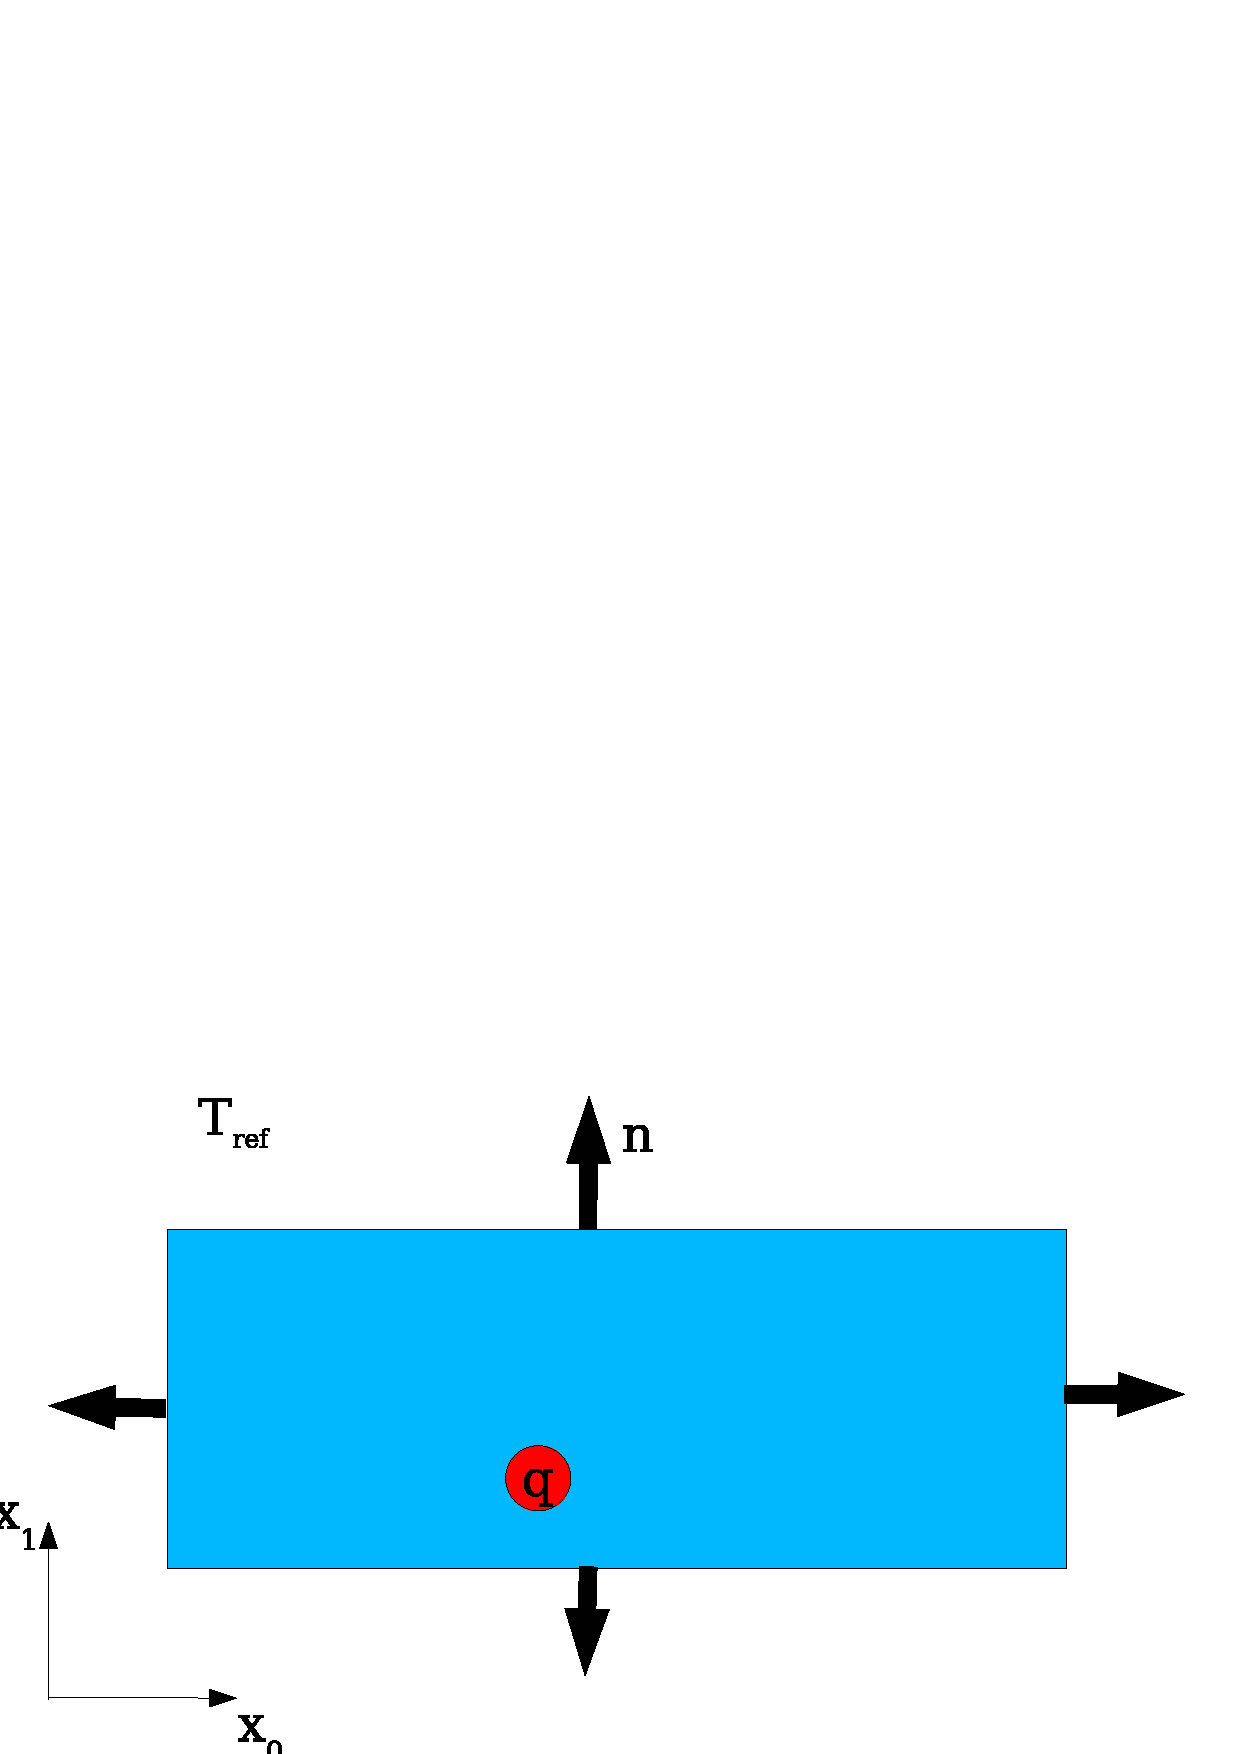
\includegraphics[width=\figwidth]{DiffusionDomain}}
% \caption{Temperature Diffusion Problem with Circular Heat Source}
% \label{WAVE FIG 1}
% \end{figure}

\begin{figure}
% \centerline{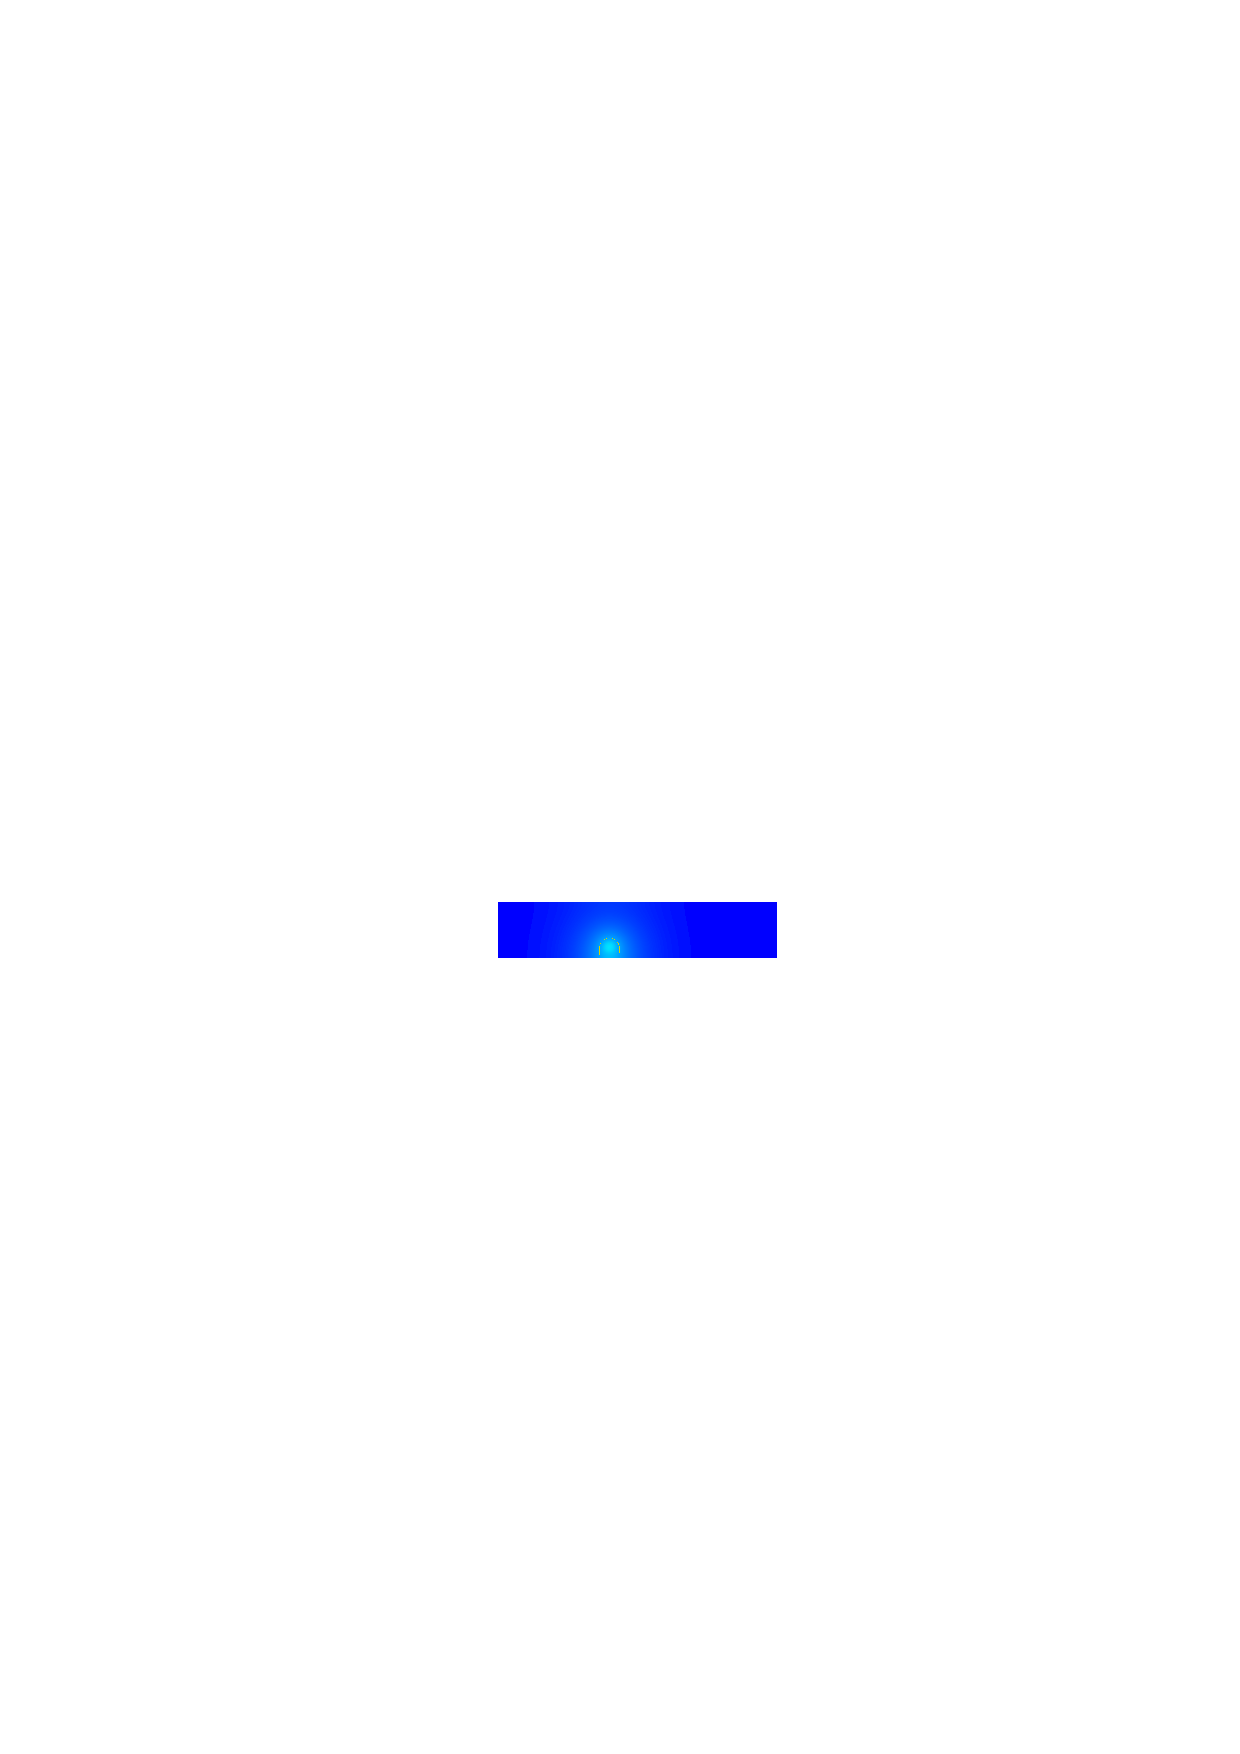
\includegraphics[width=\figwidth]{DiffusionRes1}}
% \centerline{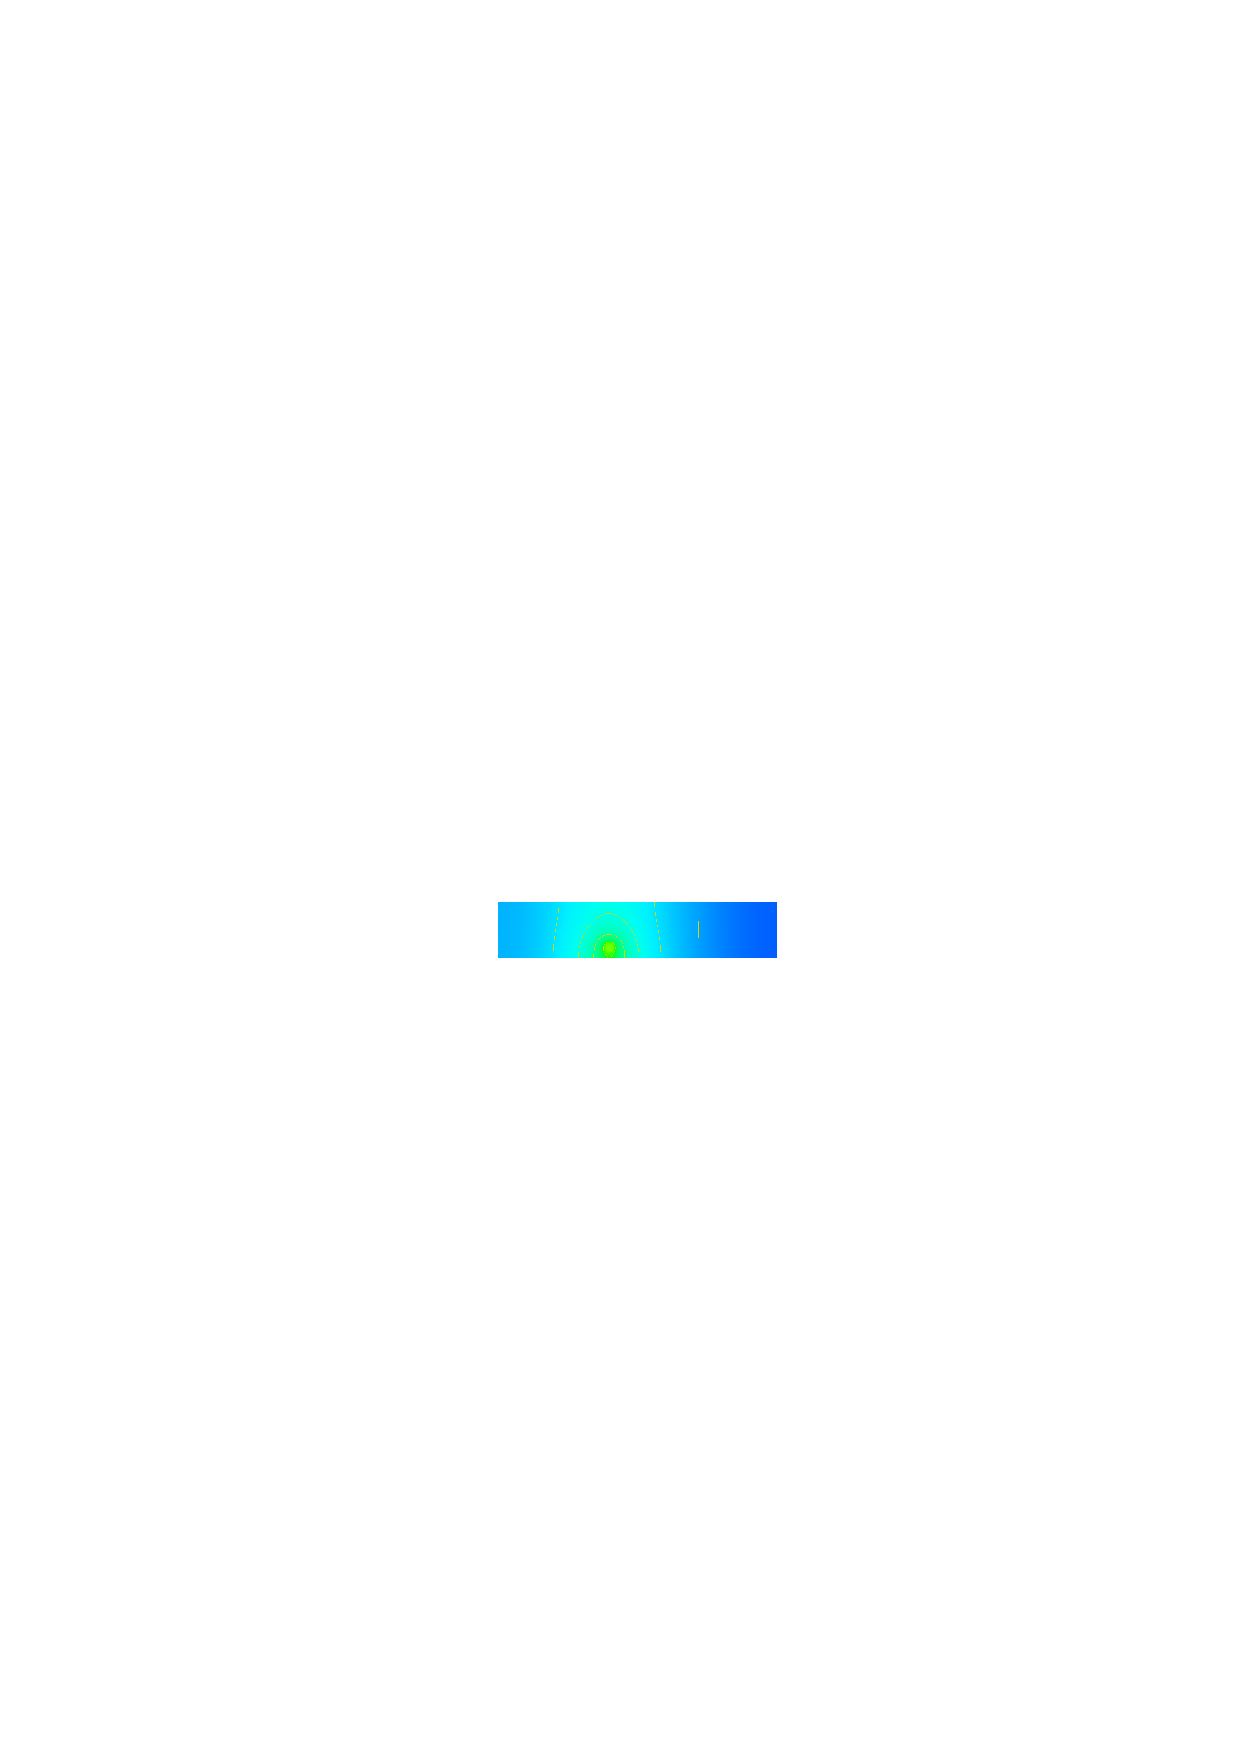
\includegraphics[width=\figwidth]{DiffusionRes16}}
% \centerline{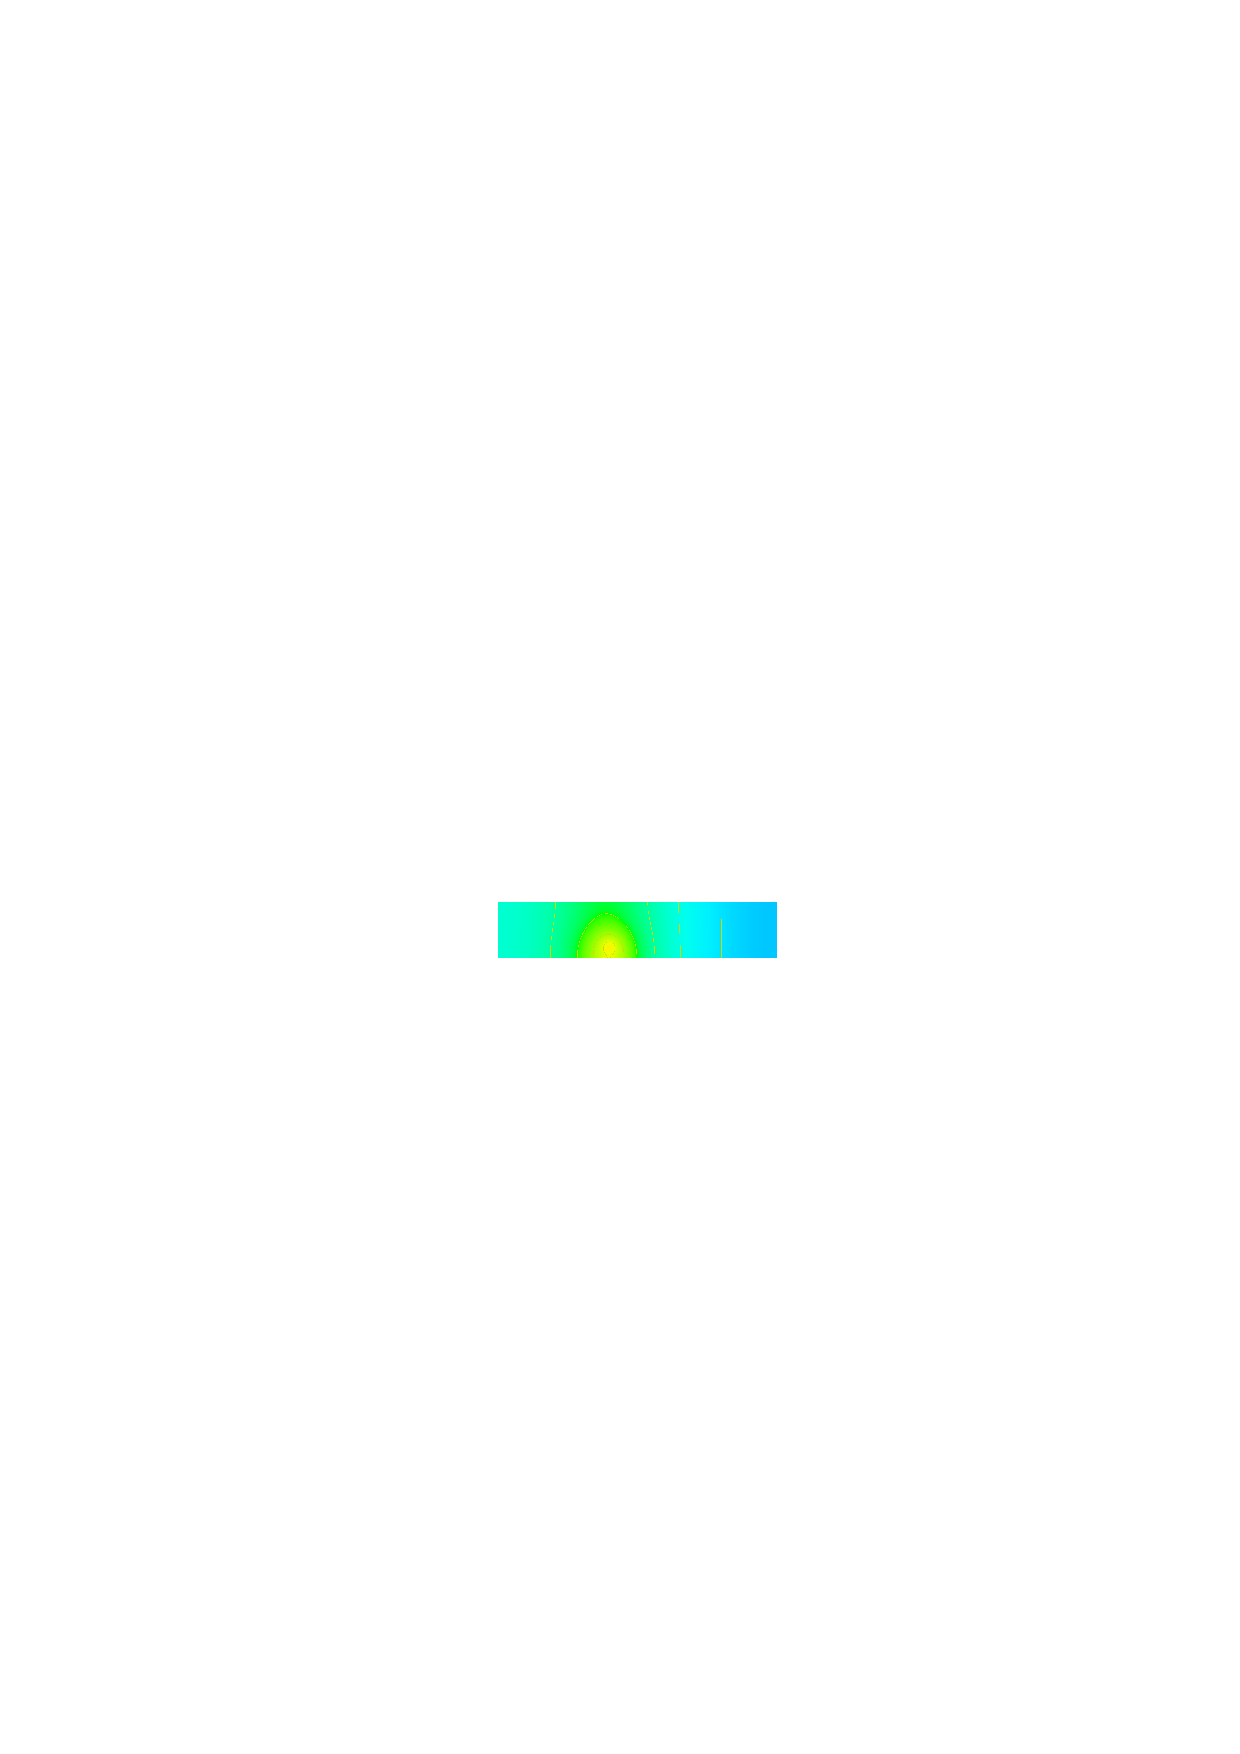
\includegraphics[width=\figwidth]{DiffusionRes32}}
%\centerline{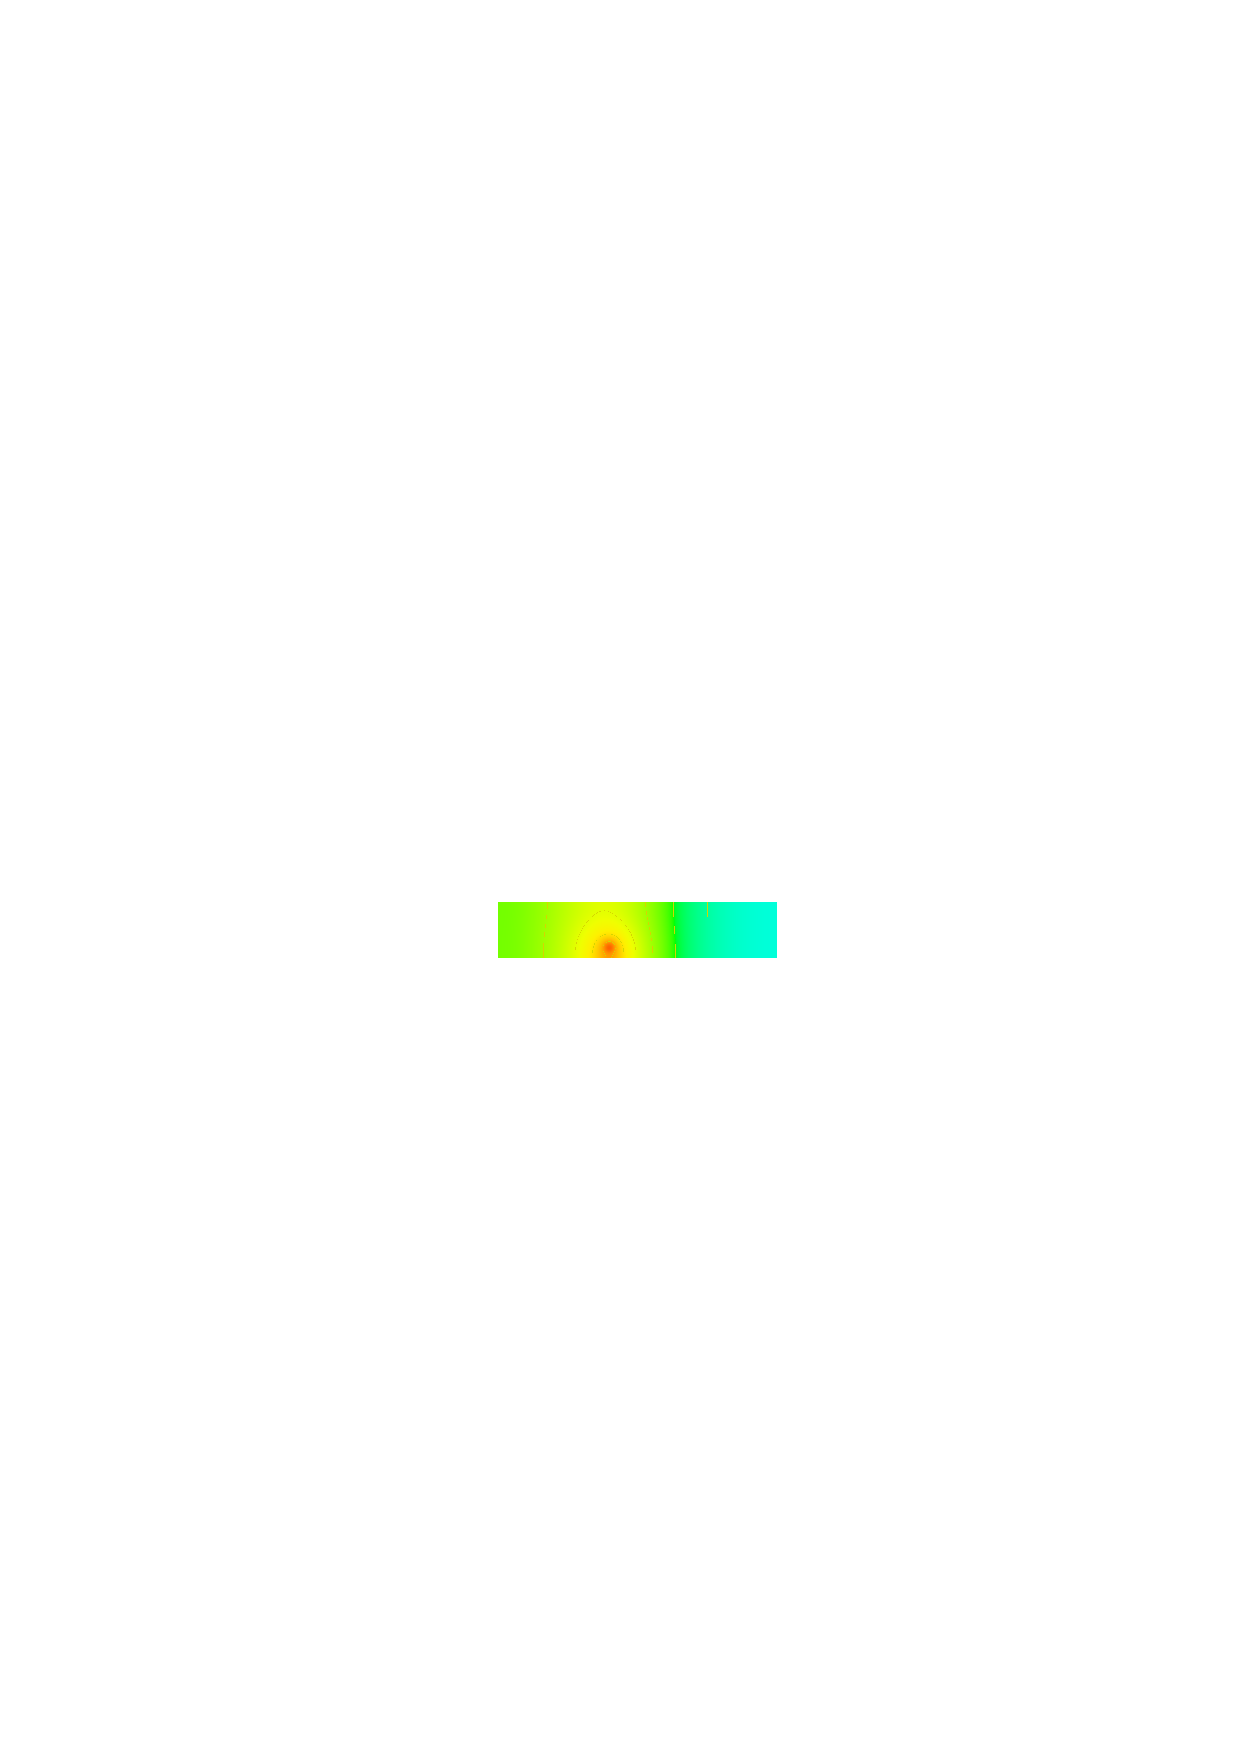
\includegraphics[width=\figwidth]{DiffusionRes48}}
\caption{Selected time steps of a wave propagation over a $10km \times 100km \times 100km$ 
with time step size $h=0.0666$. Color represents the acceleration.}
\label{WAVE FIG 2}
\end{figure}
